\chapter{Evaluación de SMMD}

Una vez instalada la apliacion de SMMD en el CECAD se mostrará a continuación sus funcionalidades principales y su manejo.

\subsection{Caso práctico CECAD}

En la figura se puede observar la creación de un dashboard personalizado el cual muestra los valores de las métricas \texttt{fibonacci-count},\texttt{fibonacci-average},\texttt{fibonacci-sum}, valores que son enviados a través de la libreria cliente de statsd en python.


\begin{figure}[h]
 \centering
  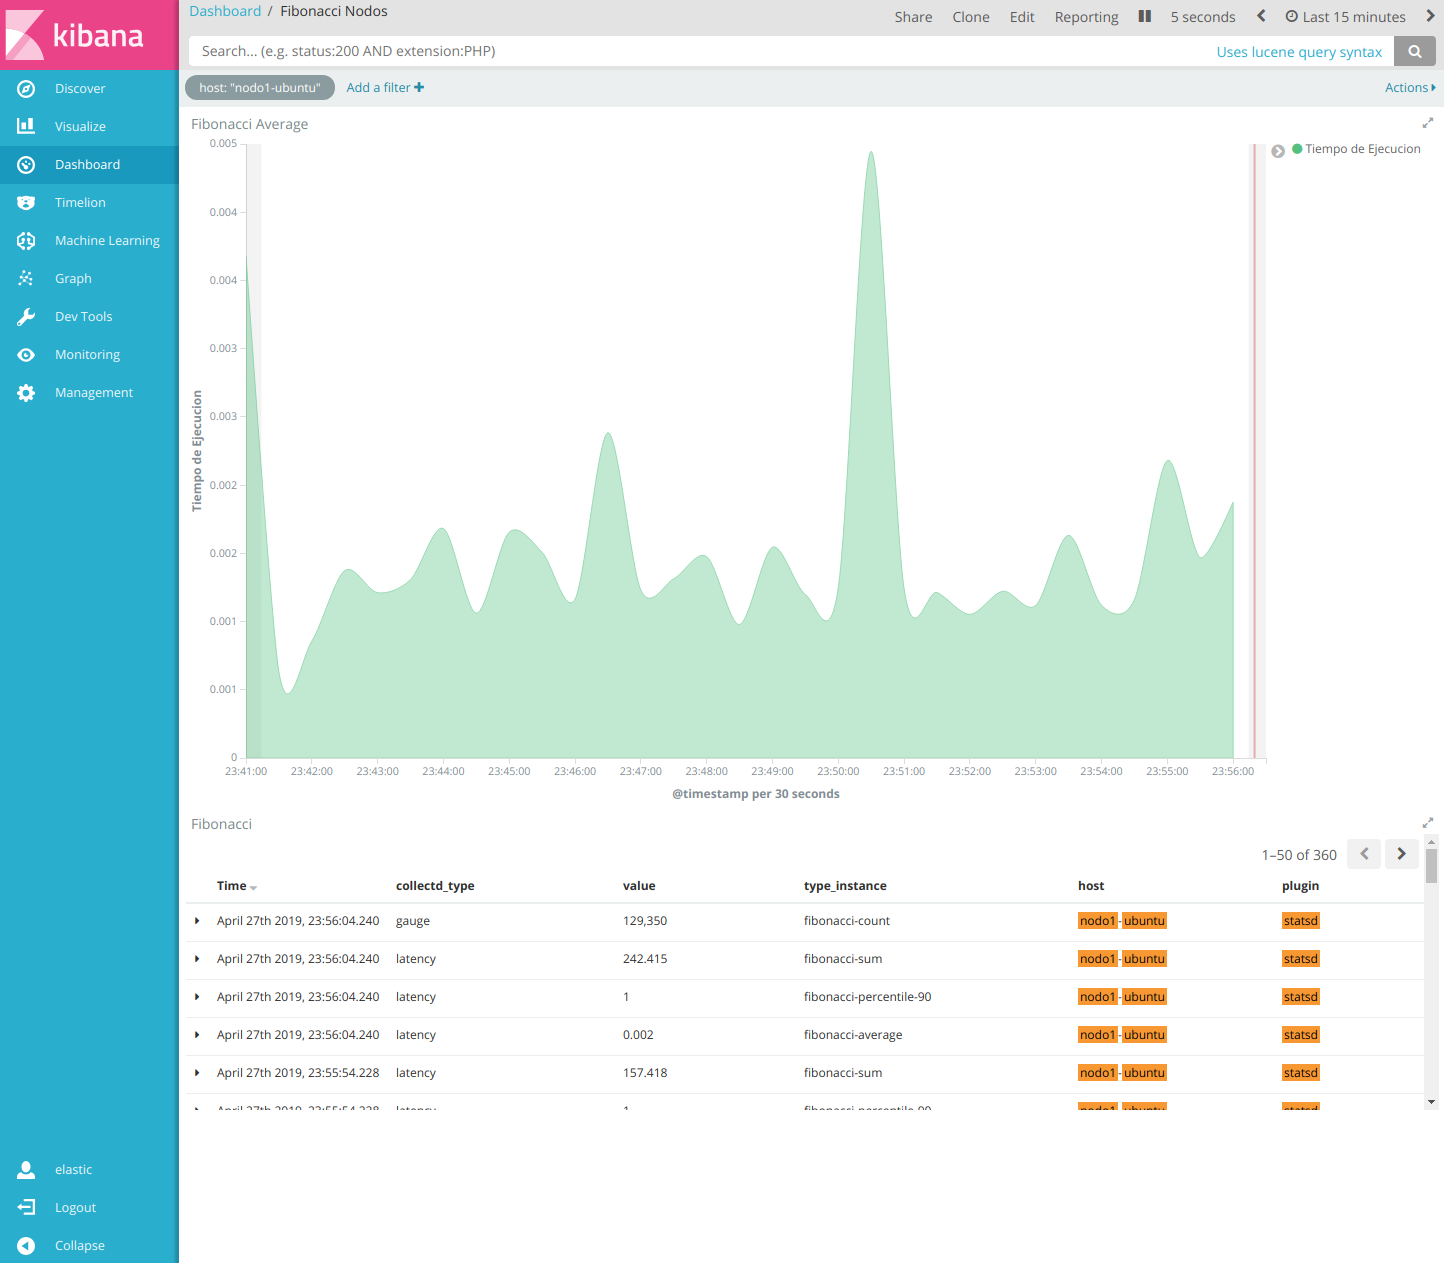
\includegraphics[width=0.8\linewidth]{./imagenes/dashboard-fibonacci.png}
  \caption{Dashboard Personalizado para la medición de métricas recibidas por StatsD}
  \label{fig:dashboard-fibonacci}
\end{figure}